\documentclass[12pt]{article}
\usepackage[english]{babel}
\usepackage[utf8]{inputenc}
\usepackage{amsmath, amssymb, amsthm}
\usepackage{graphicx}
\usepackage{hyperref}
\usepackage[margin=.75in]{geometry}
\usepackage{xcolor}
\usepackage{tikz}

\newtheorem{theorem}{Theorem}
\newtheorem{prop}{Proposition}
\newtheorem*{prop*}{Proposition}
\newtheorem{obs}{Observation}
\newtheorem*{obs*}{Observation}

\setlength{\topmargin}{0pt}
\setlength{\headsep}{0pt}
\textheight = 600pt

\title{Graph Theory \\ Homework 9}
\author{Ben Kallus and Nicholas Adair}
\date{Due Monday, Monday, March 15}

\begin{document}
\maketitle

\noindent{\bf 6.4}

{\bf (a)} $G = C_5$

{\bf (b)} $G = K_3$

{\bf (c)} $G = P_4$

{\bf (d)} $G = P_2$

{\bf (e)} $G:$
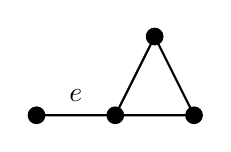
\begin{tikzpicture}
	\draw[fill=black] (0, 0) circle (3pt);
	\draw[fill=black] (1, 0) circle (3pt);
	\draw[fill=black] (2, 0) circle (3pt);
	\draw[fill=black] (1.5, 1) circle (3pt);

	\node at (.5, .25) {$e$};

	\draw[thick] (0,0) -- (1,0) -- (2,0) -- (1.5,1) -- (1,0);
\end{tikzpicture}

\newpage\noindent{\bf 6.6} Proposition: If $G$ be a connected regular graph that is not Eulerian, and $\overline{G}$ is connected, then $\overline{G}$ is Eulerian.
\begin{proof}
	Let $G$ be a connected $r$-regular graph of order $n$ that is not Eulerian such that $\overline G$ is connected.
	Since $G$ is not Eulerian, $r$ must be odd by Theorem 6.1.
	Then, by Corollary 2.3, $n$ is even.
	In any simple graph, a vertex's degree is at most $n - 1$.
	By the definition of $\overline G$, $\deg_G v + \deg_{\overline{G}} v = n - 1$.
	Thus, $$\deg_{\overline{G}} v = n - 1 - \deg_G v = n - 1 - r.$$
	Since $n$ is even and $r$ is odd, $n - 1 - r$ is even.
	Thus, every vertex of $\overline{G}$ has even degree.
	Therefore, by Theorem 6.1, $\overline{G}$ is Eulerian.
\end{proof}


\newpage\noindent{\bf 6.10} Proposition: If $G$ is a 6-regular graph of order 10, then for all $u,v \in V(G)$, $G$, $G - u$, and $G - u - v$ are all Hamiltonian.
\begin{proof}
	Let $G$ be a 6-regular graph of order 10.
	Then, $\delta(G) = 6 \geq \frac{10}2$.
	Thus, by Corollary 6.7, $G$ is Hamiltonian.

	Let $u \in V(G)$.
	Then, because $G$ is 6-regular, $G-u$ has 6 vertices of degree 5 and 3 vertices of degree 6.
	Thus, $\delta(G-u) = 5 \geq \frac{9}2$.
	Thus, by Corollary 6.7, $G-u$ is Hamiltonian.

	Let $v \in G-u$.
	Then, since $G-u$ consists only of degree 5 and 6 vertices, and contains only 3 degree-6 vertices, $v$ must be adjacent to a vertex of degree 5 in $G-u$.
	Thus, $\delta(G - u - v) = 4 \geq \frac{8}{2}$.
	Thus, by Corollary 6.7, $G-u-v$ is Hamiltonian.
\end{proof}

% You haven't yet shown that there are no cut-vertices. Just use the theorem about all paths between u and w and show that all non-adjacent vertices have a path through b and a path through c.
\newpage\noindent{\bf 6.14}

{\bf (a)}
\begin{proof} There exists a 2-connected Eulerian graph that is not Hamiltonian.
	Consider the following graph, $G$:
	\begin{center}
	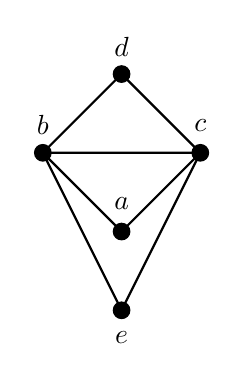
\begin{tikzpicture}
		\draw[fill=black] (0,0) circle (3pt);
		\node at (0,.35) {$b$};
		\draw[fill=black] (1,1) circle (3pt);
		\node at (1,1.35) {$d$};
		\draw[fill=black] (2,0) circle (3pt);
		\node at (2,.35) {$c$};
		\draw[fill=black] (1,-1) circle (3pt);
		\node at (1,-.65) {$a$};
		\draw[fill=black] (1,-2) circle (3pt);
		\node at (1,-2.35) {$e$};
		\draw[thick] (0,0) -- (1,1) -- (2,0) -- (1,-1) -- (0,0) -- (1,-2) -- (2,0) -- (0,0);
	\end{tikzpicture}
	\end{center}

	$G$ is clearly connected.
	By Theorem 6.1, $G$ is Eulerian.
	Suppose that $G$ does have a cut-vertex $v$.
	Then, by Theorem 5.3, there exist distinct $u,w \in V(G) \setminus \{v\}$ such that every $u-w$ path in $G$ contains $v$.
	Thus, $u$ and $w$ are not adjacent.
	Therefore, $u$ is neither $b$ nor $c$, since $b$ and $c$ are adjacent to each other vertex in $G$.
	Similarly, $w$ is neither $b$ nor $c$.
	Thus, $u,w \in \{a,d,e\}$.
	Note that $(a,c,d)$ and $(a,b,d)$ are $a-d$ paths in $G$.
	Since the inner vertices of those paths are disjoint, it cannot be that $u = a$ and $w = d$.
	Since $a, d, e$ are in symmetric positions in $G$, a symmetric argument shows that $u$ and $w$ are not both in $\{a,d,e\}$.
	Thus, no $u,w$ satisfying the condition in Theorem 5.3 exists in $G$, so $G$ does not have a cut-vertex.
	Thus, $G$ is 2-connected.

	Suppose that $G$ were Hamiltonian.
	Then, $G$ contains a Hamiltonian cycle $C$ with first edge $ab$.\footnote{Since $b$ and $c$ are in symmetric positions, the same argument applies if the cycle starts with $ac$, instead.}
	Thus, since $a$ is incident to only two edges, $C$'s last edge must be $ca$.
	Note that $C$'s second edge must be one of $bd, be, bc$.
	Suppose that $C$'s second were $bc$.
	Then, since $C$'s last edge is $ca$, and $c$ cannot be repeated in $C$, it must be that $C = (a, b, c, a)$, which is not a Hamiltonian cycle.
	Thus, $C$'s second edge cannot be $bc$.
	Now, suppose that $C$'s second edge were $bd$.
	Then, $C$'s third edge must be $dc$.
	Then, by the same logic used previously, it must be that $C = (a, b, d, c, a)$, which is not a Hamiltonian cycle.
	Since $e$ and $d$ are in symmetric positions in $G$, the same argument shows that $C$'s second edge also cannot be $be$.
	Thus, no Hamiltonian cycle exists in $G$, so $G$ is not Hamiltonian.
\end{proof}

\newpage
{\bf (b)} There exists a Hamiltonian graph that is not Eulerian and has an Eulerian complement.
\begin{proof}
	Consider the following graph, $G:$
	\begin{center}
	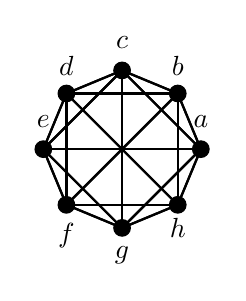
\begin{tikzpicture}
		\draw[fill=black] (1.0, 0.0) circle (3pt);
		\node at (1.0, 0.35) {$a$};
		\draw[fill=black] (0.707, 0.707) circle (3pt);
		\node at (0.707, 1.057) {$b$};
		\draw[fill=black] (0.0, 1.0) circle (3pt);
		\node at (0.0, 1.35) {$c$};
		\draw[fill=black] (-0.707, 0.707) circle (3pt);
		\node at (-0.707, 1.057) {$d$};
		\draw[fill=black] (-1.0, 0.0) circle (3pt);
		\node at (-1.0, 0.35) {$e$};
		\draw[fill=black] (-0.707, -0.707) circle (3pt);
		\node at (-0.707, -1.10) {$f$};
		\draw[fill=black] (-0.0, -1.0) circle (3pt);
		\node at (0.0, -1.35) {$g$};
		\draw[fill=black] (0.707, -0.707) circle (3pt);
		\node at (0.707, -1) {$h$};
		
		\draw[thick] (1.0, 0.0) -- (-0.0, -1.0);
		\draw[thick] (1.0, 0.0) -- (0.707, 0.707);
		\draw[thick] (1.0, 0.0) -- (-1.0, 0.0);
		\draw[thick] (1.0, 0.0) -- (0.0, 1.0);
		\draw[thick] (1.0, 0.0) -- (0.707, -0.707);
		\draw[thick] (0.707, 0.707) -- (1.0, 0.0);
		\draw[thick] (0.707, 0.707) -- (-0.707, 0.707);
		\draw[thick] (0.707, 0.707) -- (0.0, 1.0);
		\draw[thick] (0.707, 0.707) -- (-0.707, -0.707);
		\draw[thick] (0.707, 0.707) -- (0.707, -0.707);
		\draw[thick] (0.0, 1.0) -- (-0.0, -1.0);
		\draw[thick] (0.0, 1.0) -- (1.0, 0.0);
		\draw[thick] (0.0, 1.0) -- (0.707, 0.707);
		\draw[thick] (0.0, 1.0) -- (-1.0, 0.0);
		\draw[thick] (0.0, 1.0) -- (-0.707, 0.707);
		\draw[thick] (-0.707, 0.707) -- (0.707, 0.707);
		\draw[thick] (-0.707, 0.707) -- (-1.0, 0.0);
		\draw[thick] (-0.707, 0.707) -- (0.0, 1.0);
		\draw[thick] (-0.707, 0.707) -- (-0.707, -0.707);
		\draw[thick] (-0.707, 0.707) -- (0.707, -0.707);
		\draw[thick] (-1.0, 0.0) -- (-0.0, -1.0);
		\draw[thick] (-1.0, 0.0) -- (1.0, 0.0);
		\draw[thick] (-1.0, 0.0) -- (-0.707, 0.707);
		\draw[thick] (-1.0, 0.0) -- (0.0, 1.0);
		\draw[thick] (-1.0, 0.0) -- (-0.707, -0.707);
		\draw[thick] (-0.707, -0.707) -- (-0.0, -1.0);
		\draw[thick] (-0.707, -0.707) -- (0.707, 0.707);
		\draw[thick] (-0.707, -0.707) -- (-1.0, 0.0);
		\draw[thick] (-0.707, -0.707) -- (-0.707, 0.707);
		\draw[thick] (-0.707, -0.707) -- (0.707, -0.707);
		\draw[thick] (-0.0, -1.0) -- (1.0, 0.0);
		\draw[thick] (-0.0, -1.0) -- (-1.0, 0.0);
		\draw[thick] (-0.0, -1.0) -- (0.0, 1.0);
		\draw[thick] (-0.0, -1.0) -- (-0.707, -0.707);
		\draw[thick] (-0.0, -1.0) -- (0.707, -0.707);
		\draw[thick] (0.707, -0.707) -- (-0.0, -1.0);
		\draw[thick] (0.707, -0.707) -- (1.0, 0.0);
		\draw[thick] (0.707, -0.707) -- (0.707, 0.707);
		\draw[thick] (0.707, -0.707) -- (-0.707, 0.707);
		\draw[thick] (0.707, -0.707) -- (-0.707, -0.707);
	\end{tikzpicture}
	\end{center}

	Observe that $(a,b,c,d,e,f,g,h,a)$ is a Hamiltonian path in $G$.
	Thus, $G$ is Hamiltonian.
	Since $G$ is 5-regular, $G$ is not Eulerian by Theorem 6.1.
	Note that $(a,d,g,b,e,h,c,f,a)$ is an Eulerian circuit in $\overline G$, so $\overline G$ is Eulerian.

\end{proof}

\newpage\noindent{\bf 6.16} Let $G$ be a connected $r$-regular graph of even order $n$ such that $\overline G$ is connected.

{\bf (a)} Proposition: Either $G$ or $\overline G$ is Eulerian.
\begin{proof}
	Suppose that neither $G$, nor $\overline G$ is Eulerian.
	Then, since $G$ is not Eulerian, by Theorem 6.1, $r$ is odd.
	Thus, $\overline G$ is $(n-1-r)$-regular.
	Since $n-1-r$ is even, $\overline G$ must be Eulerian, which contradicts our supposition.
	Thus, either $G$ or $\overline G$ is Eulerian.
\end{proof}

{\bf (b)} Proposition: Either $G$ or $\overline G$ is Hamiltonian.
\begin{proof}
	Suppose $r \geq \frac{n}{2}$.
	Then, $\deg_G v \geq \frac{n}{2}$ for all $v \in V(G)$.
	Thus, by Dirac's Theorem, $G$ is Hamiltonian.
	Now, suppose that $r < \frac{n}{2}$.
	Then, $\deg_G v < \frac{n}{2}$ for all $v \in V(G)$.
	Thus, since $\deg_G v$ is an integer, $\deg_G v \leq \frac n2 - 1$.
	By the definition of $\overline G$, $\deg_{\overline G}v = n - \deg_Gv-1$.
	Thus, $\deg_{\overline G}v \geq n - (\frac n2 - 1) - 1 = \frac n2$.
	Therefore, by Dirac's Theorem, $\overline{G}$ is Hamiltonian.
\end{proof}

\newpage\noindent{\bf 6.20} Proposition: If $G$ is a graph of order $n \geq 3$ with the property that for each $v \in V(G)$, there is a Hamiltonian path with initial vertex $v$, then $G$ is 2-connected and not necessarily Hamiltonian.
\begin{proof}
	Let $G$ be a graph of order $n \geq 3$ with the property that for each $v \in V(G)$, there is a Hamiltonian path with initial vertex $v$.
	Thus, since $G$ has a Hamiltonian path, it is connected.
	Let $x, y \in V(G)$.
	Then, there exists a Hamiltonian path $P = (x = p_0, \hdots, p_i = y, \hdots, p_n)$ starting at $x$.
	Thus, $P' = (x = p_0, \hdots, p_i = y)$ is an $x-y$ path in $G$, so $G$ is connected.
	Suppose that $G$ does have a cut-vertex $c$.
	Then, there exist $u,w \in V(G) \setminus \{v\}$ such that all $u-w$ walks contain $c$.
	Consider a Hamiltonian path $C$ with initial vertex $c$.
	Suppose, without loss of generality, that $u$ comes before $w$ in $C$.
	Consider $C'$, the subsequence of $C$ starting at $u$ and ending at $w$.
	Since $c$ is the initial vertex of $C$, it must not be present in $C'$.
	Thus, $C'$ is a $u-w$ walk that does not contain $c$, so not all $u-w$ walks contain $c$, which contradicts our supposition.
	Thus, $G$ must have no cut-vertices.
	Thus, $G$ is 2-connected.

	Observe that $G$ need not be Hamiltonian: FIND AN EXAMPLE

\end{proof}

\newpage\noindent{\bf 6.22}

	{\bf (a)} Yes.
	\begin{proof}
		$G = K_8 \cup N_2$ is an example of such a graph.
		$G$ has ${8 \choose 2} = 28$ edges.
		Since $G$ is disconnected, it must not be Hamiltonian.
	\end{proof}

	{\bf (b)} No.
	\begin{proof}
		By the Handshaking Lemma, the sum of the degrees of $H$ is $56$.
		Since $H$ has at least 5 vertices of degree 5, and at least 3 vertices of degree of 6, the last two vertices of $H$ must have a total degree of $$56 - 5 \cdot 5 - 3 \cdot 6 = 56 - 25 - 18 = 13.$$
    		Note that $\deg v \leq 9$ for any $v \in V(H)$, since $H$ is of order 10.
    		Thus, since $H$ is not Hamiltonian, Dirac's Theorem shows that one of the unknown vertices must be of degree at most $4$.
		Suppose that one of the unknown vertices has degree $d$ less than 4.
		Then, the other unknown vertex must have degree $13 - d > 9$, which is a contradiction.
		Thus, the degrees of the unknown vertices are $4$ and $9$.
		Thus, the degree sequence of $H$ is $(9, 6, 6, 6, 5, 5, 5, 5, 5, 4)$.
    
		Let $u$ be the degree-4 vertex in $H$.
		If $u$ were connected to a vertex of degree at less than, then $H$ would be Hamiltonian by Dirac's Theorem.
		Thus, we need only consider the case in which $u$'s neighbors are exactly those vertices of degree 6 or greater.
		Let $v$ be a vertex of degree 5 in $H$.
		Then, $v$ is not adjacent to $u$.
		Thus, there are 3 vertices in $H$ of degree at least 5 that are not adjacent to $v$.
		Then, by Theorem 6.8, $H$ is Hamiltonian if and only if $H+vw$ is Hamiltonian, for some $w \in V(G)$ of degree at least 5.
		By iteratively applying this process to each vertex of degree 5 in $H$, we find that $H$ is Hamiltonian if and only if a graph with one vertex of degree 4, and 9 vertices of degree greater than or equal to 6 is Hamiltonian.
		By Ore's Theorem, such a graph is Hamiltonian, so $H$ is Hamiltonian.
		Thus, no graph exists with the desired properties.
	\end{proof}
\newpage\noindent{\bf 6.24}
    {\bf (a)}
    \begin{proof}
	Let $G$ be a graph of order $2k+1$ with $k+1$ vertices of degree 2 and $k$ vertices of degree greater than 2, such that no two vertices of degree 2 are adjacent.
	Suppose that $G$ has a Hamiltonian cycle $C$.
	Consider the Hamiltonian path $P$ obtained by removing the final edge from $C$.
	In order for $P$ to contain all $k+1$ vertices of degree 2, it must have a single vertex of degree greater than 2 between each pair of vertices of degree 2.
	Since there are $k+1$ vertices of degree 2 and $k$ vertices of degree greater than 2, $P$ must begin and end with a vertex of degree 2.
	Thus, the final edge in $C$ runs between two vertices of degree 2, which contradicts the definition of $G$.
	Thus, $G$ is not Hamiltonian.
    \end{proof}

    {\bf (b)}
    \begin{proof}
	Let $H = K_2 + N_2$.
	Then, the vertices from $K_2$ have degree $3$ and the vertices from $N_2$ have degree $2$ in $H$.
	By Dirac's Theorem, $H$ is a Hamiltonian graph.
    \end{proof}


\newpage\noindent{\bf ALSO (1)} Proposition: If $r+s<t$, then $K_{r,s,t}$ is not Hamiltonian.
\begin{proof}
	Suppose $r + s < t$.
	Consider $S$, the subgraph of $K$ induced by its partite sets of order $r$ and $s$.
	Note that $|S| = r + s$.
	Define $T$ to be the subgraph of $K$ induced by the vertices of its partite set of order $t$.
	Then, $K_{r,s,t} - S = T$.
	Note that $k(T) = t$.
	Thus, by Theorem 6.5, $K_{r,s,t}$ is not Hamiltonian.
\end{proof}

\newpage\noindent{\bf ALSO (2)} Proposition: If $r+s \geq t$, then $K_{r,s,t}$ is Hamiltonian.
\begin{proof}
	Suppose that $r+s \geq t$.
	Define $R$, $S$, $T$ to be $K_{r,s,t}$'s partite sets of orders $r,s,t$ respectively.
	
	If $|T| = 1$, then $K_{r,s,t}$ contains all possible edges between vertices in $T$.
	Let $t_1,t_2 \in T$.
	Then, $\deg(t_1) = \deg(t_2) = r + s$.
	Thus, $$\deg(t_1) + \deg(t_2) = r + s + r + s \geq r + s + t = n,$$ so $C(K_{r,s,t})$ contains the edge $t_1-t_2$.
	Thus, $C(K_{r,s,t})$ contains all possible edges between vertices in $T$.

	if $|S| = 1$, then $C(K_{r,s,t})$ contains all possible edges between vertices in $S$.
	Otherwise, let $s_1, s_2 \in S$. 
	Then, $\deg(s_1) = \deg(s_2) = r + t$.
	Thus, $$\deg(s_1) + \deg(s_2) = r + t + r + t \geq r + s + r + s \geq r + s + t = n,$$ so $C(K_{r,s,t})$ contains the edge $s_1-s_2$.
	Thus, $C(K_{r,s,t})$ contains all possible edges between vertices in $S$.

	If $|R| = 1$, then $C(K_{r,s,t})$ contains all possible edges between vertices in $R$.
	Otherwise, let $r_1, r_2 \in R$.
	Then, $\deg(r_1) = \deg(r_2) = s + t$.
	Thus, $$\deg(r_1) + \deg(r_2) = s + t + s + t \geq r + t + r + t \geq r + s + r + s \geq r + s + t = n,$$ so $C(K_{r,s,t})$ contains the edge $r_1-r_2$.
	Thus, $C(K_{r,s,t})$ contains all possible edges between vertices in $R$.

	Thus, $C(K_{r,s,t})$ is complete, so $K_{r,s,t}$ is Hamiltonian by Theorem 6.9.

\end{proof}
\end{document}
